\exercise

Given the graph $G = \left\{(a,b),\ (a,d),\ (b,c),\ (c,a),\ (c,e),\ (d,b),\
(d,e),\ (e,c) \right\}$
%
\begin{enumerate}

  \item Perform a DFS visit of $G$, specifying the edges and nodes in the order
  they are visited (assume that the adjacency list of each node is sorted by
  destination-node label).

  \item Build the MST of $G$ (assumed undirected) via Kruskal’s algorithm,
  assuming that the weight of the edge $(x,y)$ is computed as $2\times rank(x)
  \times rank(y) \bmod 7$, and $rank(x)$ is the rank in the alphabet of the
  letter $x$ or $y$, counting from 2.

\end{enumerate}

\solution

\begin{enumerate}

  \item Starting from node $a$, the visiting order is $(a,b)$, $(b,c)$, $(c,e)$,
  $(e,d)$.

  \item \autoref{tab:kruskal-cost} shows the computed cost of every edge in $G$.
  Kruskal's algorithm begins with 5 singleton sets (subforests), $S =
  \left\{\{a\},\ \{b\},\ \{c\},\ \{d\},\ \{e\}\right\}$. Then, at every step,
  extract the edge of minimum cost and, if the two nodes of the edge belong to
  different subforests, it add the edge to the final MST and unite the two
  subforests. \autoref{fig:kruskal} shows the steps computed by the algorithm.
  %
  \begin{table}[h]
    \centering
    \begin{tabular}{c|c|c|c|c}
      $x$ & $y$ & $rank(x)$ & $rank(y)$ & $c(x,y)$ \\ \hline\hline
      $c$ & $a$ & 4 & 2 & $2 \times 4 \times 2 \bmod 7 = 2$ \\
      $d$ & $b$ & 5 & 3 & $2 \times 5 \times 3 \bmod 7 = 2$ \\
      $b$ & $c$ & 3 & 4 & $2 \times 3 \times 4 \bmod 7 = 3$ \\
      $d$ & $e$ & 5 & 6 & $2 \times 5 \times 6 \bmod 7 = 4$ \\
      $a$ & $b$ & 2 & 3 & $2 \times 2 \times 3 \bmod 7 = 5$ \\
      $a$ & $d$ & 2 & 5 & $2 \times 2 \times 5 \bmod 7 = 6$ \\
      $c$ & $e$ & 4 & 6 & $2 \times 4 \times 6 \bmod 7 = 6$ \\
      $e$ & $c$ & 6 & 4 & $2 \times 6 \times 4 \bmod 7 = 6$ \\
    \end{tabular}
    \caption{Cost of every edge in graph $G$, in ascending order.}
    \label{tab:kruskal-cost}
  \end{table}
  %
  \begin{figure}[h]
    \begin{subfigure}{0.33\linewidth}
      \centering
      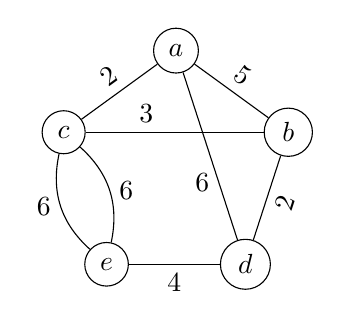
\begin{tikzpicture}
        \def \radius {1.5cm}

        \node[draw, circle] (a) at (90:\radius) {$a$};
        \node[draw, circle] (b) at (18:\radius) {$b$};
        \node[draw, circle] (c) at (162:\radius) {$c$};
        \node[draw, circle] (d) at (306:\radius) {$d$};
        \node[draw, circle] (e) at (234:\radius) {$e$};

        \path (c) edge node[sloped, above] {2} (a);
        \path (d) edge node[sloped, below] {2} (b);
        \path (b) edge node[pos=0.66, sloped, above] {3} (c);
        \path (d) edge node[sloped, below] {4} (e);
        \path (a) edge node[sloped, above] {5} (b);
        \path (a) edge node[pos=0.66, left] {6} (d);
        \path (c) edge[bend left] node[right] {6} (e);
        \path (e) edge[bend left] node[left] {6} (c);
      \end{tikzpicture}
      \caption{}
    \end{subfigure}%
    \begin{subfigure}{0.33\linewidth}
      \centering
      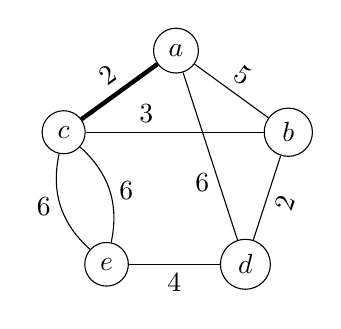
\begin{tikzpicture}
        \def \radius {1.5cm}

        \node[draw, circle] (a) at (90:\radius) {$a$};
        \node[draw, circle] (b) at (18:\radius) {$b$};
        \node[draw, circle] (c) at (162:\radius) {$c$};
        \node[draw, circle] (d) at (306:\radius) {$d$};
        \node[draw, circle] (e) at (234:\radius) {$e$};

        \path (c) edge[ultra thick] node[sloped, above] {2} (a);
        \path (d) edge node[sloped, below] {2} (b);
        \path (b) edge node[pos=0.66, sloped, above] {3} (c);
        \path (d) edge node[sloped, below] {4} (e);
        \path (a) edge node[sloped, above] {5} (b);
        \path (a) edge node[pos=0.66, left] {6} (d);
        \path (c) edge[bend left] node[right] {6} (e);
        \path (e) edge[bend left] node[left] {6} (c);
      \end{tikzpicture}
      \caption{}
    \end{subfigure}%
    \begin{subfigure}{0.33\linewidth}
      \centering
      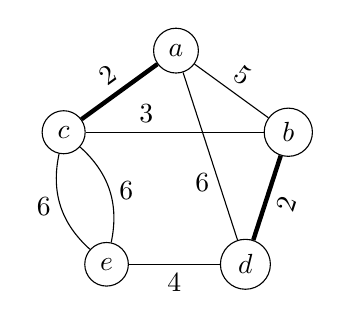
\begin{tikzpicture}
        \def \radius {1.5cm}

        \node[draw, circle] (a) at (90:\radius) {$a$};
        \node[draw, circle] (b) at (18:\radius) {$b$};
        \node[draw, circle] (c) at (162:\radius) {$c$};
        \node[draw, circle] (d) at (306:\radius) {$d$};
        \node[draw, circle] (e) at (234:\radius) {$e$};

        \path (c) edge[ultra thick] node[sloped, above] {2} (a);
        \path (d) edge[ultra thick] node[sloped, below] {2} (b);
        \path (b) edge node[pos=0.66, sloped, above] {3} (c);
        \path (d) edge node[sloped, below] {4} (e);
        \path (a) edge node[sloped, above] {5} (b);
        \path (a) edge node[pos=0.66, left] {6} (d);
        \path (c) edge[bend left] node[right] {6} (e);
        \path (e) edge[bend left] node[left] {6} (c);
      \end{tikzpicture}
      \caption{}
    \end{subfigure} \\

    \hspace{0.17\linewidth}%
    \begin{subfigure}{0.33\linewidth}
      \centering
      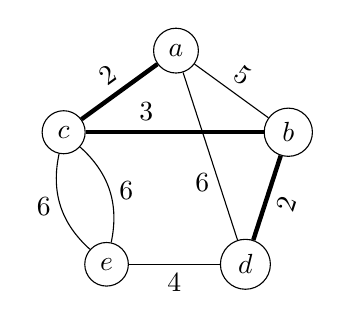
\begin{tikzpicture}
        \def \radius {1.5cm}

        \node[draw, circle] (a) at (90:\radius) {$a$};
        \node[draw, circle] (b) at (18:\radius) {$b$};
        \node[draw, circle] (c) at (162:\radius) {$c$};
        \node[draw, circle] (d) at (306:\radius) {$d$};
        \node[draw, circle] (e) at (234:\radius) {$e$};

        \path (c) edge[ultra thick] node[sloped, above] {2} (a);
        \path (d) edge[ultra thick] node[sloped, below] {2} (b);
        \path (b) edge[ultra thick] node[pos=0.66, sloped, above] {3} (c);
        \path (d) edge node[sloped, below] {4} (e);
        \path (a) edge node[sloped, above] {5} (b);
        \path (a) edge node[pos=0.66, left] {6} (d);
        \path (c) edge[bend left] node[right] {6} (e);
        \path (e) edge[bend left] node[left] {6} (c);
      \end{tikzpicture}
      \caption{}
    \end{subfigure}%
    \begin{subfigure}{0.33\linewidth}
      \centering
      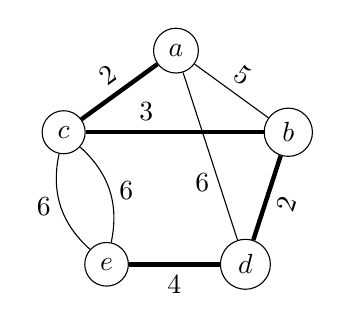
\begin{tikzpicture}
        \def \radius {1.5cm}

        \node[draw, circle] (a) at (90:\radius) {$a$};
        \node[draw, circle] (b) at (18:\radius) {$b$};
        \node[draw, circle] (c) at (162:\radius) {$c$};
        \node[draw, circle] (d) at (306:\radius) {$d$};
        \node[draw, circle] (e) at (234:\radius) {$e$};

        \path (c) edge[ultra thick] node[sloped, above] {2} (a);
        \path (d) edge[ultra thick] node[sloped, below] {2} (b);
        \path (b) edge[ultra thick] node[pos=0.66, sloped, above] {3} (c);
        \path (d) edge[ultra thick] node[sloped, below] {4} (e);
        \path (a) edge node[sloped, above] {5} (b);
        \path (a) edge node[pos=0.66, left] {6} (d);
        \path (c) edge[bend left] node[right] {6} (e);
        \path (e) edge[bend left] node[left] {6} (c);
      \end{tikzpicture}
      \caption{}
    \end{subfigure}

    \caption{Execution of Kruskal's algorithm on graph $G$. After last step, all
    nodes will be in the same subforest, and any new extracted edge will be
    irrelevant.}
    \label{fig:kruskal}
  \end{figure}

\end{enumerate}
